% Derived from PGF's geometric-shape mitered border-anchor algorithms.
\documentclass[border=2pt]{standalone}
\usepackage{tikz}
\usetikzlibrary{arrows.meta,shapes.geometric}

\begin{document}
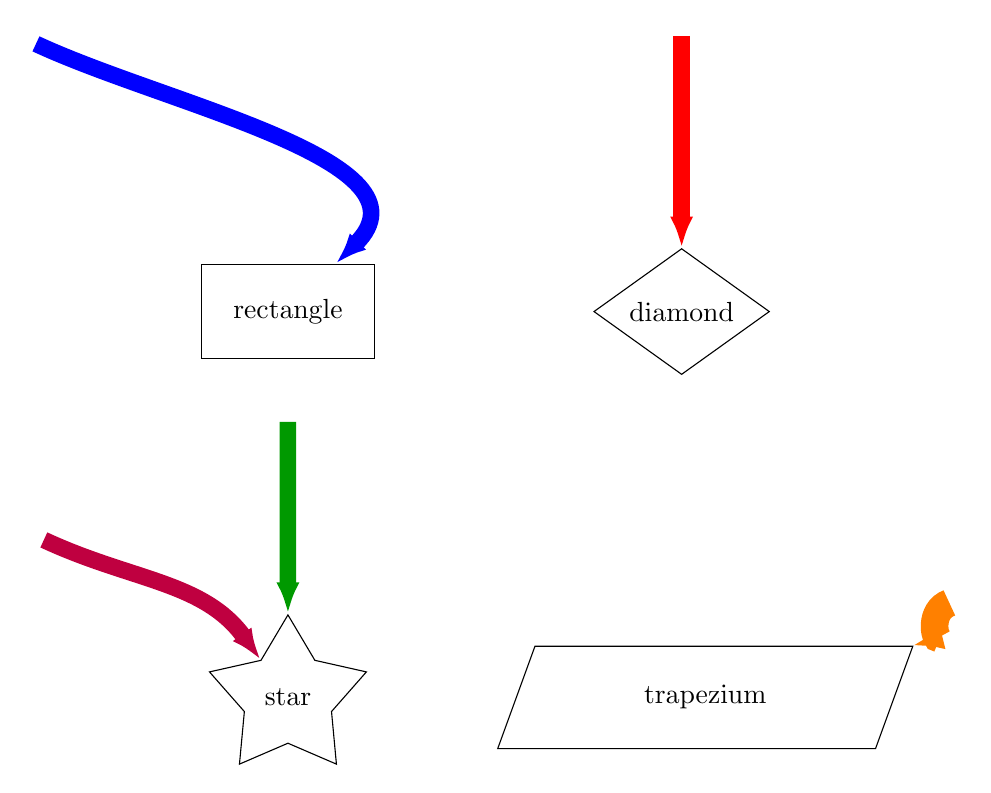
\begin{tikzpicture}[x=1cm,y=1cm]
  \node[draw,rectangle,minimum width=2.2cm,minimum height=1.2cm] (rect) at (-2,1.8) {rectangle};
  \node[draw,diamond,aspect=1.4,minimum width=2cm,minimum height=1.6cm] (diamond) at (3,1.8) {diamond};
  \node[draw,star,star points=5,star point ratio=1.8,minimum size=2cm] (star) at (-2,-3.1) {star};
  \node[draw,trapezium,trapezium left angle=70,trapezium right angle=110,minimum width=2.4cm,minimum height=1.3cm] (trap) at (3.3,-3.1) {trapezium};

  % Each incoming tangent targets a geometric corner rather than an edge.
  \draw[-{Latex[length=4mm,width=3mm]},line width=6pt,blue] (-5.2,5.2) to[out=-25,in=45] (rect);
  \draw[-{Latex[length=4mm,width=3mm]},line width=6pt,red] (3,5.3) to[out=-90,in=90] (diamond);
  \draw[-{Latex[length=4mm,width=3mm]},line width=6pt,green!60!black] (-2,0.4) to[out=-90,in=90] (star);
  % This tangent lies between the original and expanded top-right corner rays.
  % PGF therefore switches from the slanted side to the mitered top contour.
  \draw[-{Latex[length=4mm,width=3mm]},line width=10pt,orange] (6.4,-1.9) to[out=-160,in=14.5] (trap);
  \draw[-{Latex[length=4mm,width=3mm]},line width=6pt,purple] (-5.1,-1.1) to[out=-25,in=126] (star);
\end{tikzpicture}
\end{document}
